\chapter{英语}

对于英语来说并不存在语法学家编纂的学院式语法,更多是\textbf{惯用法(USAGE)},属于
\textbf{社会语言学范畴}。

《郎文英语语法大全》中所述语法指:
\begin{description}
\item [句法(SYNTAX)] 如陈述句变疑问句,句子简化或复合等。
\item [词法(MORPHOLOGY)] 单词的曲折变化(INFLECTIONS,也称词态变化 ACCIDENCE),
  如动词的过去分词、现在分词、过去式、第三人称单数等变化。
\end{description}

英语语法单位(从大到小)可分为:句
子 (SENTENCES), 分句 (CLAUSES), 短语 (PHRASES), 单词 (WORDS), 词素
(MORPHEME,如词缀、后缀、词态变化等)。

只有一个分句CLASUSES构成的句子被称为简单句 SIMPLE SENTENCES,两个或以上分句构成复句
COMPLEX 或 COMPOUND SENTENCES。

从属分句 SUBORDINATE CLASUSES 通常由一个从属连接词 (CONJUNCTION) 引导,
如 since。而且事实上也被称为状语从句(adverbial clause)。

语法等级体系中相等地位的两个或两个以上的单位,可构成一个与之性质相同的单位。这
种结构称为并列关系 (COORDINATION), 而且像从属关系一样,由一个称为连词的连接词
明确表示出来.这种连词叫并列 (COORDINATING) 连词。最常用的并列连词有 and, or
和 but。



\begin{figure}[htbp!]
  \centering
  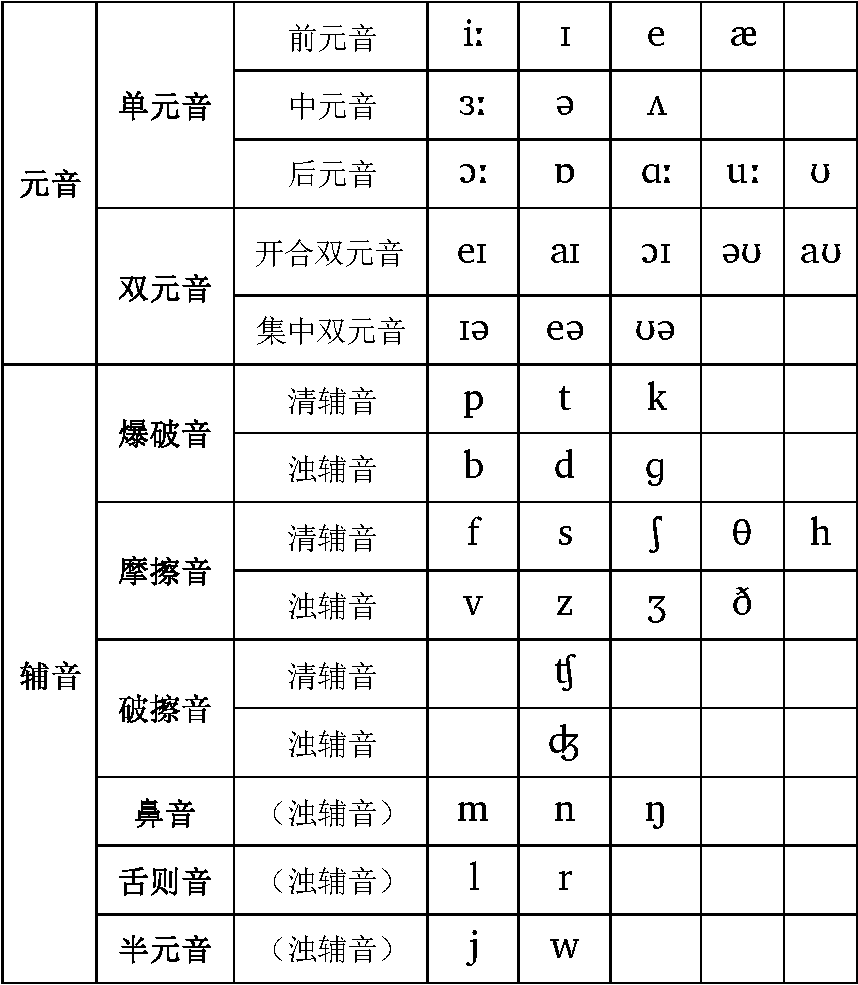
\includegraphics[width=0.8\linewidth]{gimson.pdf}
  \caption{\label{fig:gimson}Gimson英语音标}

  \bigskip

  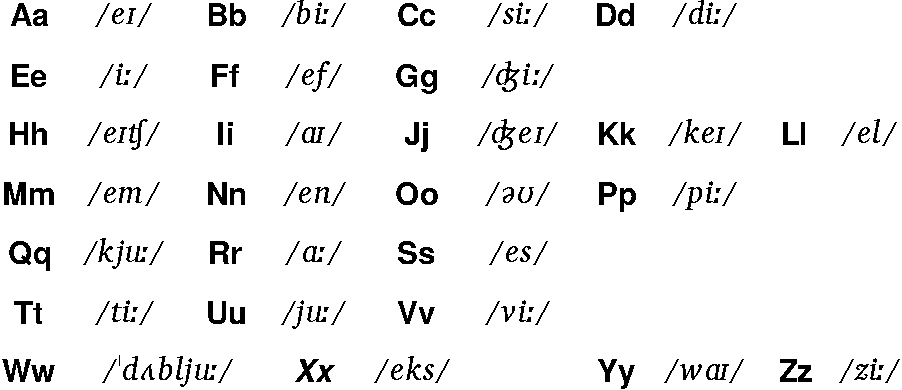
\includegraphics[width=0.8\linewidth]{alphabet.pdf}
  \caption{\label{fig:alphabet}英文字母Gimson音标}

\end{figure}

\section{动词}

根据动词在动词短语中的功能,可分为三类:
\begin{description}
\item[全义动词 FULL VERBS] 又叫实义动词 lexical verbs,如play, grow, jump等,只
  能用作主要动词。
\item[基本动词 PRIMARY VERBS] be, have, do,既可以作主要动词,也可作助动词。
\item[情态助动词 MODAL AUXILIARY VERB] may, might, will, would, can, could,
  shall, should, must,只可作为助动词,并且在动词短语中是第一个动词。


\end{description}


动词的 分词 partiple 这个名称,也反映了这一形式既带有动词特征,又带有形容词特征。


%%% Local Variables:
%%% mode: latex
%%% TeX-master: "main"
%%% End:
